\documentclass{article}
\usepackage[a4paper, total={7in, 9in}]{geometry}
\usepackage[version=3]{mhchem} % Package for chemical equation typesetting
\usepackage{siunitx} % Provides the \SI{}{} and \si{} command for typesetting SI units
\usepackage{graphicx} % Required for the inclusion of images
\usepackage{amsmath} % Required for some math elements
\usepackage{booktabs}
\usepackage{physics}
\usepackage{minted}
\usepackage{placeins}
\usepackage{subcaption}
\usepackage[english]{babel}
% Use the palatino font
\usepackage[sc]{mathpazo}

\usepackage{hyperref}
\hypersetup{%
	pdfpagelabels=true,%
	plainpages=false,%
	pdfauthor={Angus Hollands},%
	pdftitle={Year 4 MEng. Practical Monte Carlo using MCNP },%
	% pdfsubject={Determining the Velocity of Photons},% TODO
	bookmarksnumbered=true,%
	colorlinks=false,%
	citecolor=black,%
	filecolor=black,%
	linkcolor=black,% you should probably change this to black before printing
	urlcolor=black,%
	pdfstartview=FitH%
}



\setlength\parindent{0pt} % Removes all indentation from paragraphs
\DeclareSIUnit\neutron{n}
\newcommand\RT{\operatorname{RT}}

  % \renewcommand{\labelenumi}{\alph{enumi}.} % Make numbering in the enumerate environment by letter rather than number (e.g. section 6)

%\usepackage{times} % Uncomment to use the Times New Roman font

\title{Lifetime Extension Tutorial} % Title

\author{Angus \textsc{Hollands}} % Author name

\date{\today} % Date for the report

\begin{document}

\maketitle % Insert the title, author and date


\section{Part A}
In order to estimate the reference temperature safety margins for the given samples, Eq~\ref{eq:rt_ndt} and Eq~\ref{eq:rt_pts} were used.
    
    \begin{align}
    \label{eq:rt_ndt}
        \Delta{\RT}_{\operatorname{NDT}} &= R\times \operatorname{CF} \times f \\
        \RT_{\operatorname{NDT}} &= \RT(U) + \Delta\RT_{\operatorname{NDT}} + M
    \end{align}
    
    \begin{align}
    \label{eq:rt_pts}
        \Delta{\RT}_{\operatorname{PTS}} &= R\times \operatorname{CF} \times F^{0.28 - 0.10\ln{F}} \\
        \RT_{\operatorname{PTS}} &= \RT(U) + \Delta\RT_{\operatorname{PTS}} + M
    \end{align}
    
    The various parameters referenced by these equations were found as follows:
    \begin{itemize}
    \item $\sigma_\Delta$ was taken from the key (see Table~\ref{table:sigma_delta}).
    \item $M$ was calculated using Eq~\ref{eq:m}.
    \item $\operatorname{CF}$ was linearly interpolated from the chemistry tables given, using the $\ce{Cu}$ and $\ce{Ni}$ parameters given in the Charpy data source.
    \item $f$ was determined for $\Delta{\RT}_{\operatorname{NDT}}$ by mapping EOL fluence to the parameter $f$ from the digitised graph given in the specification appendix, as required.
    \end{itemize}
    
    The results for these calculations can be seen in Table~\ref{table:rt_values}. All units given in the table are consistent with those given in the report specification. It was hence determined from the PTS values that life limiting beltline materials were equally the 2-112A/C and the (second) 3-112A/C axial welds.
    
    \begin{equation}
    \label{eq:m}
        M = 2\sqrt{\sigma_U^2+\sigma_\Delta^2}
    \end{equation}

    \begin{table}[htb]
    \caption{$\sigma_\Delta$ values for different materials.}
    \label{table:sigma_delta}
    \centering
    \begin{tabular}{lr}
    \toprule
    Material &  $\sigma_\Delta$ \\
    \midrule
    Weld &  28 \\
    Base Metal &  17 \\
    \bottomrule
    \end{tabular}
    \end{table}
    
    \begin{table}
    \caption{Parameters and results from calculation of $\operatorname{RT}_{\operatorname{NDT}}$ and $\operatorname{RT}_{\operatorname{PTS}}$. The value $\Delta T\text{lim}$ denotes the temperature distance to the limiting case.}
    \label{table:rt_values}
    
    \begin{tabular}{lllrrrrrrrrr}
        \toprule
        {} &                                  Identity &              Material &  $\sigma_\Delta$ &      M &    f &     CF &  $\Delta\operatorname{RT}_{\operatorname{NDT}}$ &  $\operatorname{RT}_{\operatorname{NDT}}$  & $\Delta\operatorname{RT}_{\operatorname{PTS}}$  &  $\operatorname{RT}_{\operatorname{PTS}}$ & $\Delta T(\text{lim})$ \\
       \midrule 
        0 &   D-3803-1 &           Plate &   17 & 34.000 & 1.196 & 158.95 &  190.076 & 219.076 &  184.072 & 213.072 &   56.928 \\
        1 &   D-3803-2 &           Plate &   17 & 34.000 & 1.196 & 160.40 &  191.810 & 195.810 &  185.751 & 189.751 &   80.249 \\
        2 &   D-3803-3 &           Plate &   17 & 34.000 & 1.196 & 157.50 &  188.342 & 217.342 &  182.393 & 211.393 &   58.607 \\
        3 &   D-3804-1 &           Plate &   17 & 34.000 & 1.196 & 128.80 &  154.022 & 188.022 &  149.157 & 183.157 &   86.843 \\
        4 &   D-3804-1 &           Plate &   17 & 34.000 & 1.196 & 131.00 &  156.653 & 160.653 &  151.705 & 155.705 &  114.295 \\
        5 &   D-3804-1 &           Plate &   17 & 34.000 & 1.196 &  82.00 &   98.057 & 107.057 &   94.960 & 103.960 &  166.040 \\
        6 &  2-112A/C &      Axial Weld &   28 & 65.513 & 1.123 & 230.15 &  258.431 & 267.944 &  255.248 & 264.761 &    5.239 \\
        7 &   3-112A/C &      Axial Weld &   28 & 65.513 & 1.123 & 217.10 &  243.777 & 253.291 &  240.775 & 250.288 &   19.712 \\
        8 &   3-112A/C &      Axial Weld &   28 & 65.513 & 1.123 & 230.15 &  258.431 & 267.944 &  255.248 & 264.761 &    5.239 \\
        9 &      9-112 &  Circumf...Weld &   28 & 65.513 & 1.205 & 225.20 &  271.458 & 280.972 &  262.019 & 271.532 &   28.468 \\
        \bottomrule
        \end{tabular}
    \end{table}
    
\section{Part B}
    
    The \ce{Cu} content at the \SI{95}{\percent} probability given by the normal distribution $\mathcal{N}(\mu=\SI{0.213}{wt\percent C}, \sigma=\SI{0.02}{wt\percent C})$ was found to be \SI{0.24590}{wt\percent C}, using \mintinline[python3]{python}{scipy.stats.norm.ppf(.95, mu, std)}. The calculations performed above were then repeated, with the limiting material composition modified to this value. The results of this calculation can be seen in Table~\ref{table:rt_values_modified}. These results indicate that unless the copper content is known with sufficient accuracy, the reference safety margins should consider the case in which the copper content is underestimated. Increasing the copper content in this case would indicate that the component in question would not be safe to use, according to the safety reference limits.
    
    
    \begin{table}
    \caption{Parameters and results from calculation of $\operatorname{RT}_{\operatorname{NDT}}$ and $\operatorname{RT}_{\operatorname{PTS}}$, using modified compositions. The value $\Delta T\text{lim}$ denotes the temperature distance to the limiting case.}
    \label{table:rt_values_modified}
    
    \begin{tabular}{lllrrrrrrrrr}
        \toprule
        {} &                                  Identity &              Material &  $\sigma_\Delta$ &      M &    f &     CF &  $\Delta\operatorname{RT}_{\operatorname{NDT}}$ &  $\operatorname{RT}_{\operatorname{NDT}}$  & $\Delta\operatorname{RT}_{\operatorname{PTS}}$  &  $\operatorname{RT}_{\operatorname{PTS}}$ & $\Delta T(\text{lim})$ \\
       \midrule
0 &   D-3803-1 &           Plate &   17 & 34.000 & 1.196 & 158.950 &  190.076 & 219.076 &  184.072 & 213.072 &   56.928 \\
1 &   D-3803-2 &           Plate &   17 & 34.000 & 1.196 & 160.400 &  191.810 & 195.810 &  185.751 & 189.751 &   80.249 \\
2 &   D-3803-3 &           Plate &   17 & 34.000 & 1.196 & 157.500 &  188.342 & 217.342 &  182.393 & 211.393 &   58.607 \\
3 &   D-3804-1 &           Plate &   17 & 34.000 & 1.196 & 128.800 &  154.022 & 188.022 &  149.157 & 183.157 &   86.843 \\
4 &   D-3804-1 &           Plate &   17 & 34.000 & 1.196 & 131.000 &  156.653 & 160.653 &  151.705 & 155.705 &  114.295 \\
5 &   D-3804-1 &           Plate &   17 & 34.000 & 1.196 &  82.000 &   98.057 & 107.057 &   94.960 & 103.960 &  166.040 \\
6 &  2-112 A/C &      Axial Weld &   28 & 65.513 & 1.123 & 242.809 &  272.645 & 282.159 &  269.287 & 278.801 &   -8.801 \\
7 &   3-112A/C &      Axial Weld &   28 & 65.513 & 1.123 & 217.100 &  243.777 & 253.291 &  240.775 & 250.288 &   19.712 \\
8 &   3-112A/C &      Axial Weld &   28 & 65.513 & 1.123 & 242.809 &  272.645 & 282.159 &  269.287 & 278.801 &   -8.801 \\
9 &      9-112 &  Circumf...Weld &   28 & 65.513 & 1.205 & 225.200 &  271.458 & 280.972 &  262.019 & 271.532 &   28.468 \\
\bottomrule
        \end{tabular}
    \end{table}
        
    
    
    
\section{Part C}
    Each data set from the collection given in the specification was fit with a sigmoid function of the form
    \begin{equation}
    \label{eq:sigmoid}
        E=a + b\tanh{\frac{T-T_0}{c}}\,.
    \end{equation}
    The value for $T_{\SI{40}{\joule}}$ was then determined from the inverse sigmoid function 
    \begin{equation}
        c\operatorname{atanh}{\frac{E-a}{b}}\,,
    \end{equation}
    using these fit parameters. The $T_{\SI{40}{\joule}}$ could not be determined for the \textit{RPV 515} sample, as the upper asymptote fell below the \SI{40}{\joule} threshold. In terms of safety, it should be assumed that for all temperatures, the Charpy impact energy will be below \SI{40}{\joule} for this sample.
    
    The value $\Delta T_{\SI{40}{\joule}}$ was then determined for each data set as the difference of $T^i_{\SI{40}{\joule}}$ and $T^0_{\SI{40}{\joule}}$, the individual and unirradiated start of life parameters respectively (see Table~\ref{table:estimated_t}).
    
    Finally, a dose damage relationship function of the form 
    \begin{align}
    \label{eq:dose_damage}
    \Delta T_{\SI{40}{\joule}} &= A+B F_T\sqrt{D_{\text{eff}}} \\
    F_t &= 1.2 - 0.00106T_{\text{irr}}\,,
    \end{align}
    was fit to the irradiated and doubly irradiated groups using a linear least squares solver with a residual function (see Fig~\ref{fig:single_dose}, Fig~\ref{fig:double_dose}), and the parameters tabulated per\textendash group (see Table~\ref{table:fit_params_dose}). To handle doubly irradiated samples, it was assumed that the irradiation process is linear, and hence the expression $F_T\sqrt{D_eff}$ was replaced with the sum of that from each dose. The fit values were tabulated in see Table~\ref{table:estimated_t}. In an exploration of the research surrounding the Charpy test for irradiated samples, it was found that a particular form of the dose damage relationship outlined above may be used to maximise the a likelihood function whose form permits the inclusion of both the single and doubly irradiated data sets into the solving procedure. It was, however, outside of the scope of this project. It was observed in the double dose group that in plotting the fit and estimated values for $\Delta T_{\SI{40}{\joule}}$, a slightly curved could be observed. This suggests that the fit function does not correctly model the data, as expected.
    
    \begin{table}[htb]
    \caption{Estimated $T_{\SI{40}{\joule}}$ and relative $T_{\SI{40}{\joule}}$ from data set.}
    \label{table:estimated_t}
    
    \begin{tabular}{lrrrrrrrrrrrr}
    \toprule
    {} &             A &       B &       C &      $T_0$ &  $D^T_1$ &  $D^F_1$ &  $T_1$ &  $D^T_2$ &  $D^F_2$ &  $T_2$ &    $T_{\SI{40}{\joule}}$ &   $\Delta T_{\SI{40}{\joule}}$ \\
    Series                   &        &        &        &        &                 &              &                            &                 &              &                            &        &        \\
    \midrule
    Start of Life     &  61.52 &  37.87 &  29.26 &  26.73 &             0.0 &          0.0 &                        0.0 &             0.0 &          0.0 &                        0.0 &   7.85 &    0.0 \\
    RPV 515           &  17.21 &  18.16 &  38.62 &   8.97 &            36.1 &         6.09 &                      198.0 &             0.0 &          0.0 &                        0.0 &    nan &    nan \\
    RPV 514           &  47.81 &   34.1 &   3.44 &  93.87 &            66.5 &          8.5 &                      198.0 &             0.0 &          0.0 &                        0.0 &  93.06 &  85.21 \\
    RPV 508           &  160.0 & 145.99 &  22.53 & 101.96 &            71.3 &         0.34 &                      190.0 &             0.0 &          0.0 &                        0.0 &  75.76 &  67.91 \\
    RPV 14            &  40.88 &  33.48 &  43.35 &  77.16 &            84.7 &        11.78 &                      198.0 &             0.0 &          0.0 &                        0.0 &  76.03 &  68.18 \\
    RPV 510           &  36.55 &  29.85 &  69.11 &  82.46 &            89.0 &        27.61 &                      198.0 &             0.0 &          0.0 &                        0.0 &  90.49 &  82.64 \\
    RPV 13            &  42.93 &  19.27 &   1.15 & 124.58 &           102.3 &         14.7 &                      198.0 &             0.0 &          0.0 &                        0.0 &  124.4 & 116.55 \\
    RPV 12            &  53.02 &  38.37 &   41.6 &  94.95 &           105.5 &        26.89 &                      198.0 &             0.0 &          0.0 &                        0.0 &  80.25 &   72.4 \\
    RPV 507           &  53.18 &  43.51 &  75.19 &  87.78 &           110.4 &         0.54 &                      190.0 &             0.0 &          0.0 &                        0.0 &  64.28 &  56.42 \\
    RPV 512           &  45.47 &  36.54 &  77.56 & 152.14 &           141.1 &        30.97 &                      198.0 &             0.0 &          0.0 &                        0.0 & 140.45 & 132.59 \\
    RPV 513           &   46.8 &  23.52 &  25.62 & 137.31 &           149.9 &        24.75 &                      198.0 &             0.0 &          0.0 &                        0.0 & 129.69 & 121.84 \\
    RPV 511           &  40.77 &  20.64 &  16.43 & 152.73 &           159.6 &        38.29 &                      198.0 &             0.0 &          0.0 &                        0.0 & 152.12 & 144.27 \\
    RPV 7             &  35.37 &  30.58 &  55.58 & 104.69 &           180.3 &         0.87 &                      190.0 &             0.0 &          0.0 &                        0.0 & 113.17 & 105.32 \\
    RPV 506           &  43.37 &  26.52 &  29.99 & 103.86 &           184.5 &         0.87 &                      190.0 &             0.0 &          0.0 &                        0.0 & 100.03 &  92.18 \\
    RPV 10            & 185.74 & 197.53 & 233.96 &  350.0 &           186.1 &        45.85 &                      198.0 &             0.0 &          0.0 &                        0.0 & 128.76 & 120.91 \\
    RPV 502           &  35.03 &  35.44 &  72.77 &  103.8 &           228.7 &         1.33 &                      190.0 &             0.0 &          0.0 &                        0.0 & 114.08 & 106.23 \\
    RPV 503           &  57.68 &  30.39 &  39.62 & 177.68 &           265.6 &         1.33 &                      190.0 &             0.0 &          0.0 &                        0.0 & 151.33 & 143.48 \\
    RPV 504           &  43.76 &  17.62 &  12.82 & 127.61 &           275.1 &         1.33 &                      190.0 &             0.0 &          0.0 &                        0.0 & 124.83 & 116.98 \\
    I20L(B)           &  36.63 &  17.62 &   0.02 & 121.02 &           105.5 &        26.89 &                      198.0 &           668.0 &         47.9 &                      189.0 & 121.02 & 113.17 \\
    I20L(B)...Set &  30.36 &  26.06 &  84.43 & 184.93 &           105.5 &        26.89 &                      198.0 &           668.0 &         47.9 &                      189.0 & 217.69 & 209.84 \\
    I30B\_1            & 132.87 & 135.01 & 339.22 & 477.02 &           141.1 &        30.97 &                      198.0 &           901.0 &         45.0 &                      280.0 & 190.73 & 182.88 \\
    I20(H)B\_1         & 174.62 & 221.87 & 537.38 &  602.0 &           141.1 &        30.97 &                      198.0 &           943.0 &         61.7 &                      186.0 &  223.8 & 215.95 \\
    I20(H)T\_1         &  40.21 &   35.5 & 101.31 & 224.26 &           141.1 &        30.97 &                      198.0 &           981.0 &         59.6 &                      188.0 & 223.66 & 215.81 \\
    I30A\_1            & 129.87 &  114.8 & 166.16 & 403.67 &           141.1 &        30.97 &                      198.0 &          1005.0 &         46.4 &                      286.0 & 228.76 &  220.9 \\
    513\_3             &    0.0 & 132.64 &  450.0 &  56.71 &           149.9 &        24.75 &                      198.0 &           369.0 &         22.6 &                      311.0 & 196.78 & 188.93 \\
    I20L(T)\_1         &  36.25 &  19.62 &  54.75 & 217.79 &           149.9 &        24.75 &                      198.0 &           693.0 &         44.8 &                      190.0 & 228.38 & 220.53 \\
    513\_2             &  600.0 & 579.57 & 102.83 & 470.28 &           149.9 &        24.75 &                      198.0 &           765.0 &         44.6 &                      292.0 &  261.3 & 253.44 \\
    103\_1             &    0.0 &   72.6 & 102.01 & 105.74 &           154.5 &        29.85 &                      198.0 &           761.0 &         42.9 &                      260.0 & 168.97 & 161.12 \\
    10\_3              &  27.37 &  33.46 &  53.19 & 108.29 &           189.6 &         1.12 &                      190.0 &           157.0 &          9.7 &                      275.0 &  129.4 & 121.55 \\
    28\_3              &  37.57 &  15.93 &  30.75 & 152.34 &           192.1 &         1.12 &                      190.0 &           436.0 &         23.6 &                      282.0 & 157.06 & 149.21 \\
    71\_2              &  42.23 &  17.18 &  25.84 & 182.15 &           207.7 &         1.12 &                      190.0 &           853.0 &         46.5 &                      273.0 & 178.77 & 170.92 \\
    I25H(B)           &   35.0 &  25.24 & 104.04 &  208.4 &           237.7 &         1.22 &                      190.0 &           902.0 &         59.6 &                      227.0 & 229.28 & 221.43 \\
    I30A\_2            &   30.6 &  23.72 &  75.81 & 172.86 &           237.7 &         1.22 &                      190.0 &          1005.0 &         46.4 &                      286.0 & 204.65 & 196.79 \\
    I20L(T)\_2        &  31.45 &   26.7 &  77.61 & 170.92 &           241.0 &         1.22 &                      190.0 &           693.0 &         44.8 &                      190.0 & 196.67 & 188.82 \\
    I20H(B)\_2         &  31.31 &  26.74 &  65.01 & 189.78 &           241.0 &         1.22 &                      190.0 &           943.0 &         61.7 &                      186.0 & 211.69 & 203.84 \\
    I20H(T)\_2         &  35.11 &  32.03 &  83.88 & 232.89 &           265.6 &         1.33 &                      190.0 &           981.0 &         59.6 &                      188.0 & 245.81 & 237.96 \\
    I30B\_2            &  34.43 &  21.09 &  60.72 & 156.65 &           275.1 &         1.33 &                      190.0 &           901.0 &         45.0 &                      280.0 & 173.09 & 165.24 \\
    I25(H)T          &  31.61 &  32.28 & 140.03 & 153.02 &           275.1 &         1.33 &                      190.0 &           946.0 &         58.5 &                      242.0 & 190.29 & 182.43 \\
    \bottomrule
    \end{tabular}
    \end{table}
        
    \begin{table}
    \centering
    \caption{Dose damage relationship fit parameters (see Eq~\ref{eq:dose_damage}).}
    \label{table:fit_params_dose}
    
    \begin{tabular}{lrr}
        \toprule
        {} &      A &     B \\
        Group  &        &       \\
        \midrule
        Single &  2.547 & 8.360 \\
        Double & 28.125 & 3.473 \\
        \bottomrule
        \end{tabular}
    \end{table}
\begin{figure}[t]
\caption{Plot of single dose $\Delta T_{\SI{40}{\joule}}$ against fit using Eq~\ref{eq:dose_damage}.}
\label{fig:single_dose}
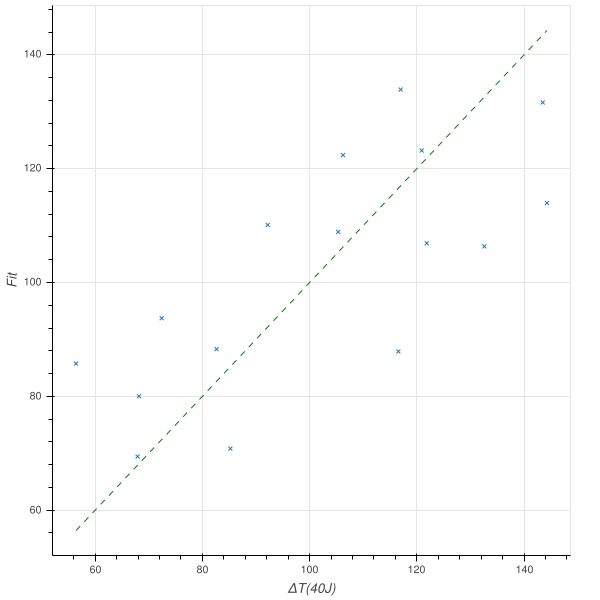
\includegraphics[width=\textwidth]{plots/single_dose.png}
\centering
\end{figure}

\begin{figure}[t]
\caption{Plot of double dose $\Delta T_{\SI{40}{\joule}}$ against fit using Eq~\ref{eq:dose_damage}.}
\label{fig:double_dose}
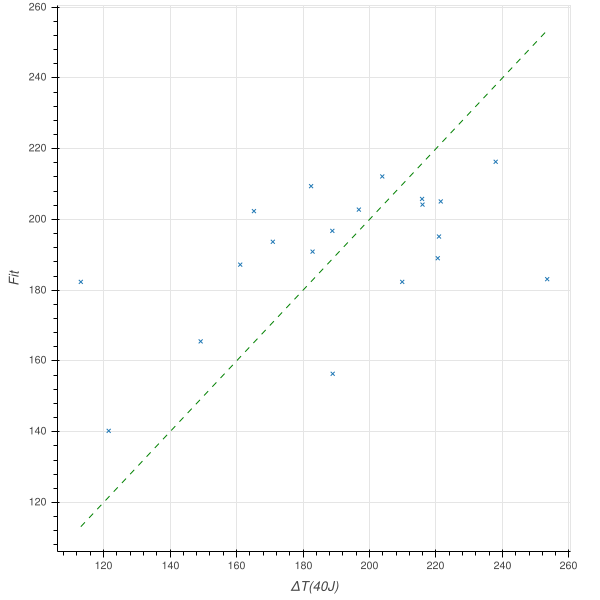
\includegraphics[width=\textwidth]{plots/double_dose.png}
\centering
\end{figure}
        
%\section{Appendix}
    %\captionof{listing}{Exercise 1. MCNP input file.\label{lst:ex_1}}
    %\inputminted[linenos,breaklines]{lexer.py -x}{mcnp/1.ip}
    
% \printbibliography

\end{document}